
%% ****** Start of file apstemplate.tex ****** %
%%
%%
%%   This file is part of the APS files in the REVTeX 4 distribution.
%%   Version 4.1r of REVTeX, August 2010
%%
%%
%%   Copyright (c) 2001, 2009, 2010 The American Physical Society.
%%
%%   See the REVTeX 4 README file for restrictions and more information.
%%
%
% This is a template for producing manuscripts for use with REVTEX 4.0
% Copy this file to another name and then work on that file.
% That way, you always have this original template file to use.
%
% Group addresses by affiliation; use superscriptaddress for long
% author lists, or if there are many overlapping affiliations.
% For Phys. Rev. appearance, change preprint to twocolumn.
% Choose pra, prb, prc, prd, pre, prl, prstab, prstper, or rmp for journal
%  Add 'draft' option to mark overfull boxes with black boxes
%  Add 'showpacs' option to make PACS codes appear
%  Add 'showkeys' option to make keywords appear

\documentclass[aps,pre,preprint,groupedaddress, floatfix]{revtex4-1}


\input ../inputs/setupSveZha
\input ../inputs/editsDasbuch   %% editing comments, DasBuch style
\input ../inputs/def            %% do not edit; update from dasbuch/book/inputs/def.tex
\input ../inputs/defsSveZha     %% all diffusion project edits: \renewcommand, etc


% You should use BibTeX and apsrev.bst for references
% Choosing a journal automatically selects the correct APS
% BibTeX style file (bst file), so only uncomment the line
% below if necessary.
%\bibliographystyle{apsrev4-1}

\begin{document}

% Use the \preprint command to place your local institutional report
% number in the upper righthand corner of the title page in preprint mode.
% Multiple \preprint commands are allowed.
% Use the 'preprintnumbers' class option to override journal defaults
% to display numbers if necessary
%\preprint{}

%Title of paper
\title{Diffuse globally, compute locally: a cyclist tale}

% repeat the \author .. \affiliation  etc. as needed
% \email, \thanks, \homepage, \altaffiliation all apply to the current
% author. Explanatory text should go in the []'s, actual e-mail
% address or url should go in the {}'s for \email and \homepage.
% Please use the appropriate macro foreach each type of information

% \affiliation command applies to all authors since the last
% \affiliation command. The \affiliation command should follow the
% other information
% \affiliation can be followed by \email, \homepage, \thanks as well.
\author{Tingnan Zhang, Daniel I. Goldman and Predrag Cvitanovi\'c}
\email[corresponding to: ]{predrag@gatech.edu}
%\homepage[]{Your web page}
%\thanks{}
%\altaffiliation{}
\affiliation{School of Physics, Georgia Institute of Technology}

%Collaboration name if desired (requires use of superscriptaddress
%option in \documentclass). \noaffiliation is required (may also be
%used with the \author command).
%\collaboration can be followed by \email, \homepage, \thanks as well.
%\collaboration{}
%\noaffiliation

\date{\today}

\begin{abstract}
\input abstract
\end{abstract}

% insert suggested PACS numbers in braces on next line
\pacs{}
% insert suggested keywords - APS authors don't need to do this
%\keywords{}

%\maketitle must follow title, authors, abstract, \pacs, and \keywords
\maketitle

% body of paper here - Use proper section commands
% References should be done using the \cite, \ref, and \label commands

\section{Introduction}

The advances in the theory of dynamical systems have brought a new life to
Boltzmann's mechanical formulation of statistical mechanics. Sinai, Ruelle and
Bowen (SRB) have generalized Boltzmann's notion of ergodicity for a constant
energy surface for a Hamiltonian system in equilibrium to dissipative systems in
{nonequilibrium} stationary states. In this more general setting the attractor
plays the role of a constant energy surface, and the SRB measure x is a
generalization of the Liouville measure. Such measures are purely microscopic
and indifferent to whether the system is at equilibrium, close to equilibrium or
far from it.  ``Far for equilibrium'' in this context refers to systems with
large deviations from Maxwell's equilibrium velocity distribution. Furthermore,
the theory of dynamical systems has yielded new sets of microscopic dynamics
formulas for macroscopic observables such as diffusion constants, to which we turn now.
%
%%%%%%%%%%%%%%%%%%%%%%%%%%%%%%%%%%%%%%%%%%%%%%%%%%%%%%%%%%%%%%%%%%
%\SFIG{fig_lor_4}
%{}{
%Deterministic diffusion in a
%finite horizon periodic Lorentz gas.
%\hfill (T. Schreiber)
%}{fig-lor-4}
%%%%%%%%%%%%%%%%%%%%%%%%%%%%%%%%%%%%%%%%%%%%%%%%%%%%%%%%%%%%%%%%%%
%

Chaotic motions exist in many field of physics systems, blah. Thre are physical
problems such as beam defocusing in particle accelerators or chaotic behavior of
passive tracers in $2$\dmn\ rotating flows which can be described as
deterministic diffusion in periodic arrays. In the field of animal/robotic
locomotion, we will show that a macroscopic ``diffusion view'' also applies.

Lately, there has been an increased focus on locomotion in complex environments. Researches in the physical sciences and in the field of robotics all find interest/relevance to this topic. (Now we can have a list of reference and recent studies in this topic). Many of those studies uses substrates that are spatially homogeneous and we have a relatively good understanding of it. Little is understood for locomotion in heterogeneous environment and principles are still lacking. Our lab is interested to study the transport properties of locomotors moving on heterogeneous terrain. Such study may potentially be beneficial to practical applications such mars navigation, hazardous rescue.

We consider the following locomotion problem. A passively controlled robot is moving in a boulder field at constant speed. We would want to study the long term dynamics of the system. The diffusion coefficient, which describes roughly how much area the robot explored in a unit time, is the key quantity here. We may place the boulder in a regular, periodic array and assume that we are in the heavy boulder limit such that after each collision event, only the robot is deflected and boudlers remain immobalized. With these preasumptions we effectively created a lorentz gas model for locomotion in a boulder field.

We shall apply cycle expansions to the analysis of {\em transport} properties of
chaotic systems. The resulting formulas are exact; no probabilistic assumptions
are made, and the all correlations are taken into account by the inclusion of
cycles of all periods.  The infinite extent systems for which the periodic orbit
theory yields formulas for diffusion and other transport coefficients are
spatially periodic, the global {\statesp} being tiled with copies of a
elementary cell.

In \refsect{s-DiffPerArr} we derive the formulas for diffusion
coefficients in a simple physical setting, the $2$\dmn\ periodic Lorentz
gas in elementary cell. In\refsect{s-SymmetryReduction} we consider further the rotational symmetry of the Lorentz gas system and derive the diffusion coefficients in fundamental domain.

\section{Diffusion in periodic arrays}
\label{s-DiffPerArr}

\begin{figure}[htbp]
\begin{center}
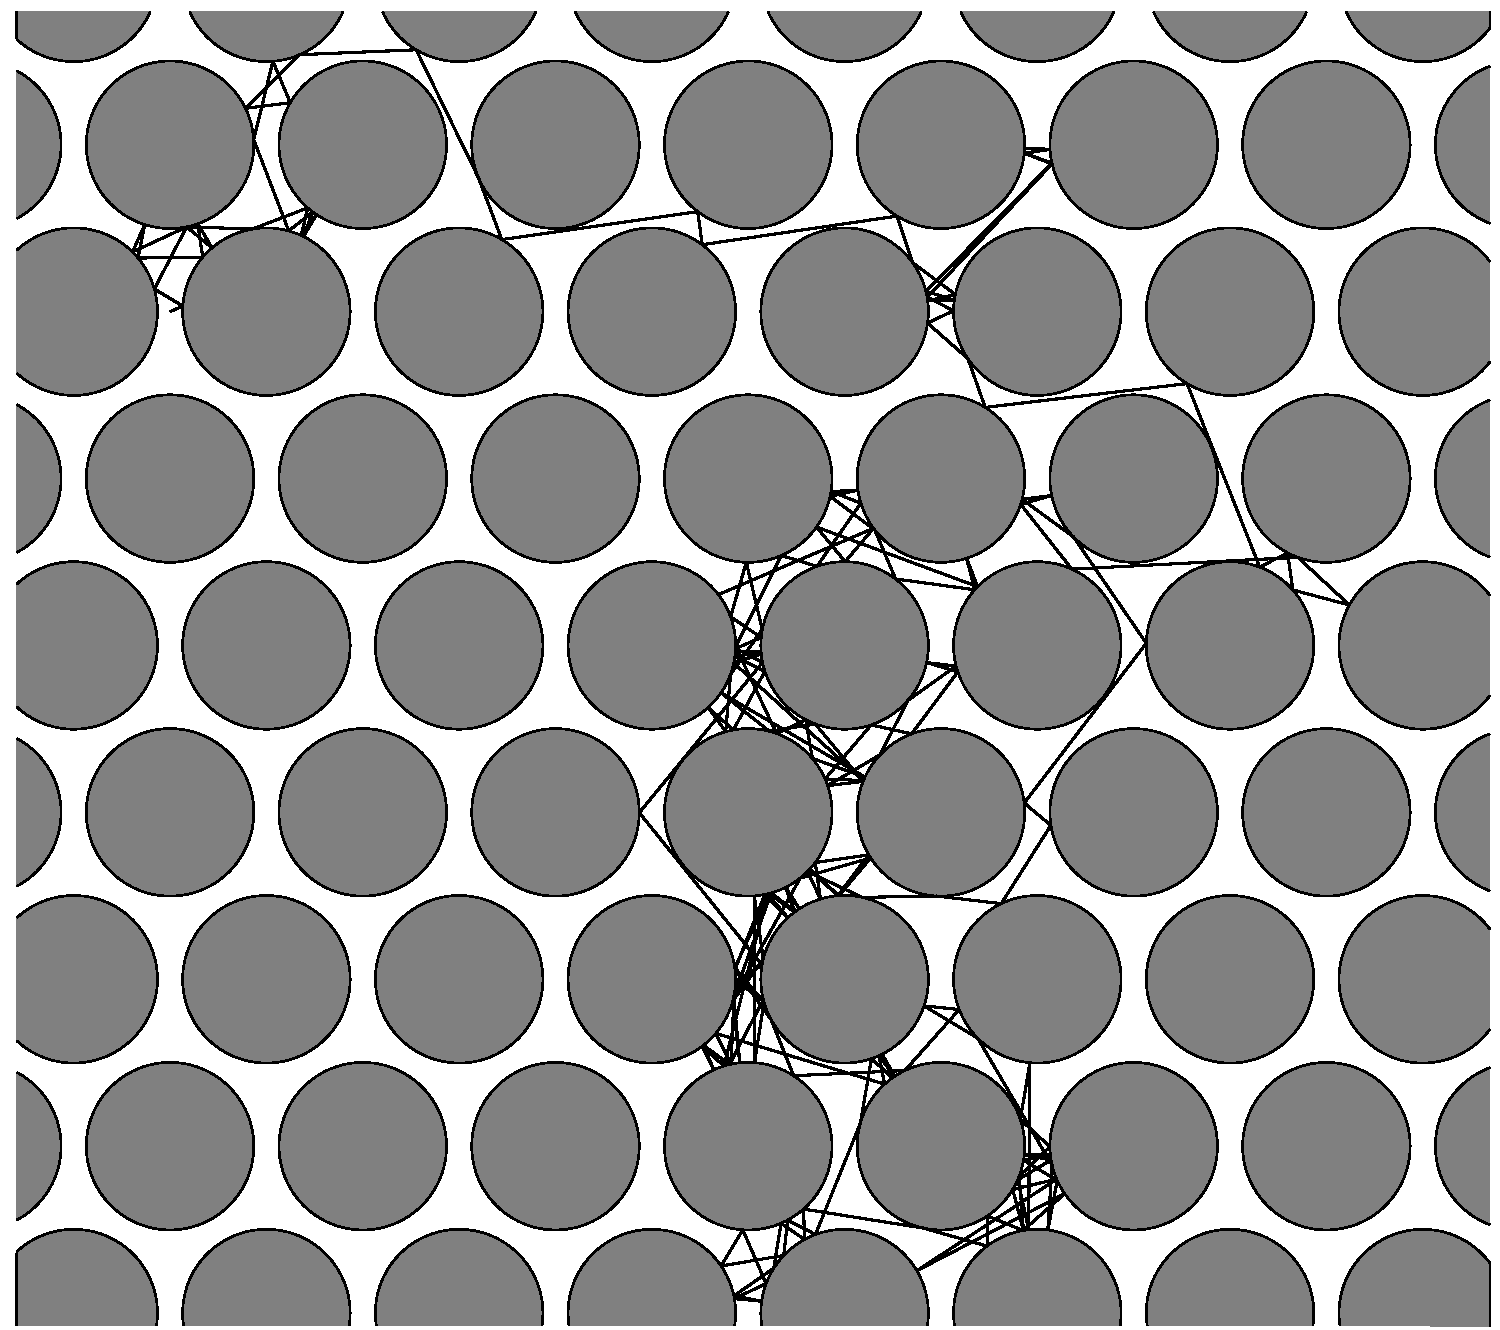
\includegraphics[width=0.8\textwidth]{diffuseChaoticBouncing}
\end{center}
\caption[]{\label{fig:chaoticBouncing} Chaotic, diffusive boucing of a particle in an array of disks. }
\end{figure}

\begin{figure}[htbp]
\begin{center}
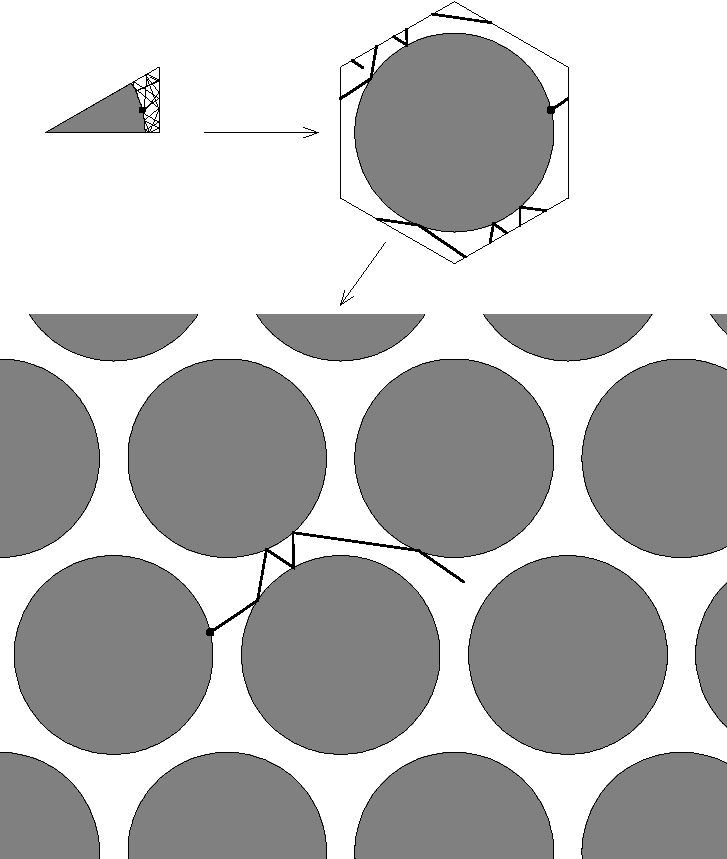
\includegraphics[width=0.45\textwidth]{diffuseSchreiberFig1}
\end{center}
\caption[]{\label{fig:schrieberFig1}Motion in fundamental domain (FD), elementary cell (EC) and full space.}

\end{figure}

The $2$\dmn\ Lorentz gas is an infinite scatterer array in which
diffusion of a light molecule in a gas of heavy scatterers is modeled
by the motion of a point particle in a plane bouncing off an array of
reflecting disks.  The Lorentz gas is called ``gas'' as one can
equivalently think of it as consisting of any number of pointlike fast
``light molecules'' interacting only with the stationary ``heavy
molecules'' and not among themselves.  As the scatterer array is built
up from only defocusing concave surfaces, it is a pure hyperbolic
system, and one of the simplest nontrivial dynamical systems that
exhibits deterministic diffusion, \reffig{fig:chaoticBouncing}.

% The original Lorentz gas assumed a random distribution of heavy
% scatterers; in this case a probabilistic description is unavoidable.

We shall now show that the {\em periodic} Lorentz gas is amenable to a
purely deterministic treatment.  In this class of open dynamical
systems quantities characterizing global dynamics, such as the
Lyapunov exponent, pressure and diffusion constant, can be computed
from the dynamics restricted to the elementary cell.  The method
applies to any hyperbolic dynamical system that is a periodic tiling
$\hM=\bigcup_{ \hn \in T} \pS_{\hn}$ of the dynamical {\statesp} $\hM$
by {\em translates} $\pS_{\hn}$ of an {\em elementary cell} $\pS$,
with $T$ the abelian group of lattice translations.  If the scattering
array has further discrete symmetries, such as reflection symmetry,
each elementary cell may be built from a {\em fundamental domain}
${\widetilde \pS}$ by the action of a discrete (not necessarily
abelian) group $G$.  The symbol $\hM$ refers here to the full
{\statesp}, \ie,, both the spatial coordinates and the momenta.  The
spatial component of $\hM$ is the complement of the disks in the {\em
whole} space.

We shall now relate the dynamics in $\pS$ to diffusive properties of
the Lorentz gas in $\hM$.

These concepts are best illustrated by a specific example, a Lorentz
gas based on the hexagonal lattice Sinai billiard of
\reffig{fig:schrieberFig1}.

We distinguish two types of diffusive behavior; the {\em infinite
horizon} case, which allows for infinite length flights, and the {\em
finite horizon} case, where any free particle trajectory must hit a
disk in finite time. 

As we will work with three kinds of \statesp s, good manners require
that we repeat what tildes, nothings and hats atop symbols signify:
\bea
\tilde{\ }     &&
    \mbox{fundamental domain, triangle in \reffig{fig:schrieberFig1}}
        \continue
%[nothing] \qquad \qquad &&
[0pt] \qquad \qquad &&
    \mbox{elementary cell, hexagon in \reffig{fig:schrieberFig1}}
        \continue
\hat{\ }   &&
    \mbox{full {\statesp}, lattice in \reffig{fig:schrieberFig1}}
\label{atops}
\eea
It is convenient to define an \evOper\ for each of the 3 cases of
\reffig{fig-lor-1}.
$\hx(t)\,=\,\hflow{t}{\hx}$
denotes the point in the global space
$\hM$
reached by the flow in time $t$.
$x(t)\,=\,\flow{t}{\xInit}$
denotes the corresponding flow in the elementary cell; the two are
related by
\beq
\hn_t(\xInit)= \hflow{t}{\xInit} - \flow{t}{\xInit} \in T
\,,
\ee{l-diff-hatn}
the translation of the endpoint of the global path into the elementary
cell $\pS$.  The quantity $\tx(t)\,=\,\tflow{t}{\tx}$ denotes the flow
in the fundamental domain
${\widetilde \pS}$;
$\tflow{t}{\tx}$ is related to
$\flow{t}{\tx}$ by a discrete symmetry
$g \in G$ which maps $\tx(t)\in {\widetilde \pS}$ to
${x}(t) \in {\pS}$ .

Fix a vector $\beta \in \reals^d$, where $d$ is the dimension of the
{\statesp}. We will compute the diffusive properties of the Lorentz
gas from the leading eigenvalue of the
\evOper\ \refeq{(2)}
\beq
\eigenvL(\beta)\,=\, \lim_{t \rightarrow \infty} \frac{1}{t} \log
\langle e^{\beta \cdot (\hx(t) -x) } \rangle_\pS
~, \quad
\ee{lor-diff-1}
where the average is over all initial points in the elementary cell,
$x \in \pS$. %, $\tx \in {\widetilde \pS}$ respectively.

If all odd derivatives vanish by symmetry, there is no drift and the
second derivatives
\[
2d D_{ij} =
\left . {{\partial} \over {\partial \beta_i}}
{{\partial} \over {\partial \beta_j}}
\eigenvL(\beta)\right |_{\beta=0} \,=\,\lim_{t\rightarrow \infty} {1\over t}
\langle {(\hx(t) -x)_i (\hx(t) -x)_j } \rangle_\pS ~,
\] %ee{lor-diff-4}
yield a diffusion matrix.  This symmetric matrix can, in general, be
anisotropic (\ie, have $d$ distinct eigenvalues and eigen\-vectors).
The spatial diffusion constant is then given by the Einstein relation
\refeq{(5)}
\[
D\,=\,{1\over 2 d} \sum_i
\left .{{\partial}^2 \over {\partial \beta^2_i}}
\eigenvL(\beta)\right |_{\beta=0}
\,=\, \lim_{t\rightarrow \infty} {1\over{2d t}}
\langle {(\hat{q}(t) -q)^2 } \rangle_\pS~
~,
\] %ee{lor_diff_5}
where the $i$ sum is restricted to the spatial components $q_i$ of the
{\statesp} vectors $x=(q,p)$, \ie, if the dynamics is Hamiltonian, the
sum is over the $d$ degrees of freedom.

PC{reinstate mass, velocity, size to get $\beta$, $m$, $\sigma$
    dependencies right}

We now turn to the connection between \refeq{lor-diff-1} and periodic
orbits in the elementary cell.As the full $\hM \rightarrow {\widetilde
\pS}$ reduction is complicated by the non-abelian nature of $G$, we


\section{Into fundamental domain}
\label{s-SymmetryReduction}

\begin{figure}
\begin{center}
(a)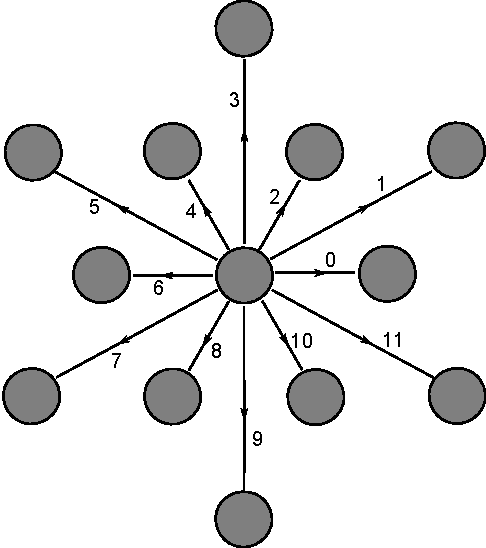
\includegraphics[width=0.29\textwidth]{diffuseDiskDirectionsElCell}
(b)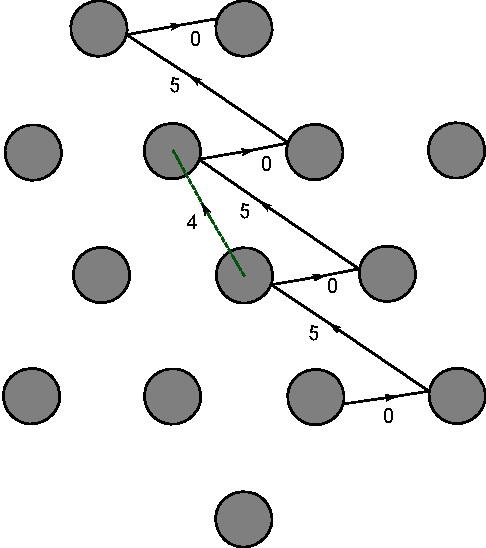
\includegraphics[width=0.29\textwidth]{diffuseDiskDirecsElCell05}
(c)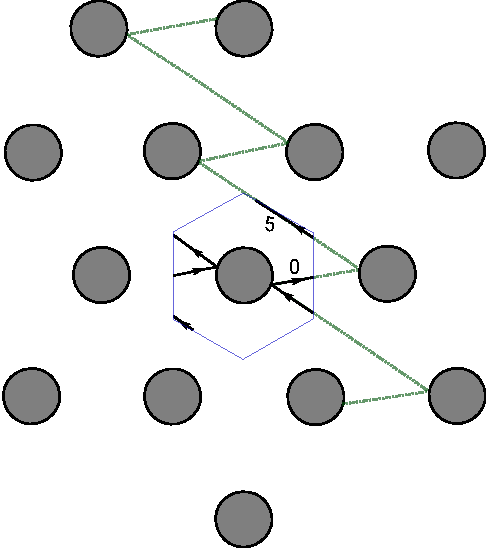
\includegraphics[width=0.29\textwidth]{diffuseDiskDirecsElCell05red}
\end{center}
\caption{
Elementary cell symbolic dynamics is obtained by labeling the translation
vectors connecting the center of the current disk to the center of the
next disk.
(a) The finite horizon is here imposed by limiting jumps from the
center cell to only the short jumps (six even labels $0, 2,\cdots,10$)
and the `long jumps' (six odd labels $1, 3,\cdots,11$).
(b) Running mode \cycle{05} advances by $\hn_4$ per period.
(c) In the elementary cell this is a \po\ \cycle{05}
    of topological length 2.
    }
\label{diskDirectionsElCell}
\end{figure}


\begin{figure}[htbp]
\begin{center}
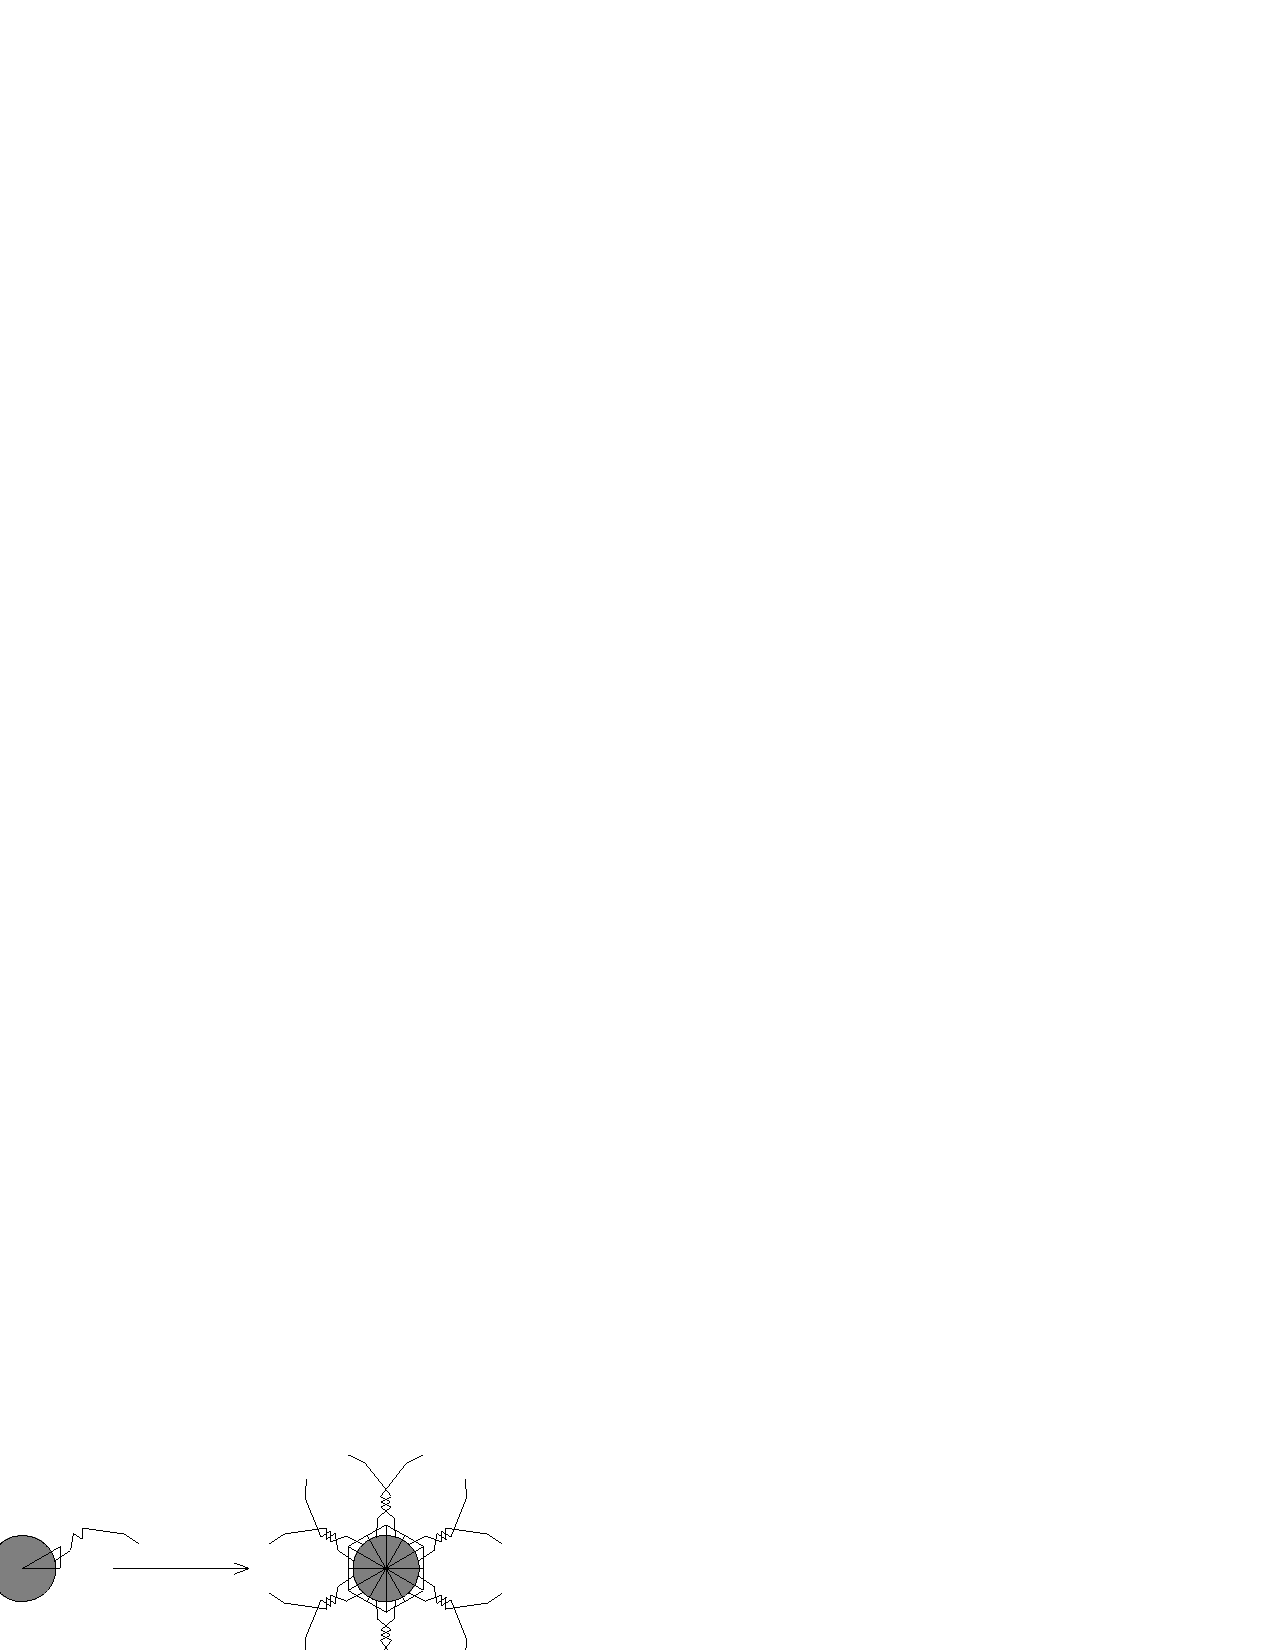
\includegraphics[width=0.45\textwidth]{diffuseSchreiberFig2}
\end{center}
\caption[]{ \label{fig:schrieberFig2}
An (unwrapped) trajectory (in full space) and its 12 copies after
applying point group actions to it.}
\end{figure}

\begin{figure}[htbp]
\begin{center}
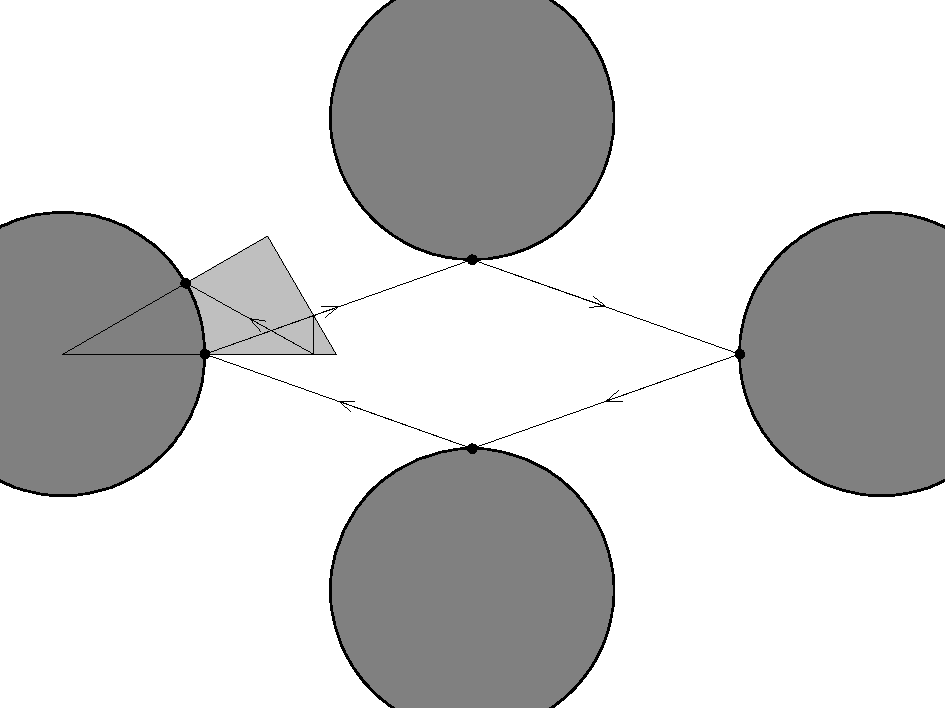
\includegraphics[width=0.45\textwidth]{diffuseSchreiberFig3}
\caption[]{Multiplicity of periodic orbits in FD. \label{fig:schrieberFig3}}
\end{center}

\end{figure}
\subsubsection{Grammar of FD cycle}
\begin{figure}
\begin{center}
(a) \includegraphics[width=0.45\textwidth]{7diskFundDflips}
(b) \includegraphics[width=0.45\textwidth]{7diskFundDtiles}
\end{center}
\caption{\label{fig:7diskFundDflips}
(a) The three generators of tiling of the plane by a fundamental domain:
two generators of \Dn{12} tiling, reflection $s$ across the short
disk-disk separation, reflection  $\ell$  across the long disk-disk
separation;
and
a translation generator $f$ that pivots (`flips') a disk center to disk
center by flip across the symmetry line normal to the short disk-disk
separation.
(5) Tiling of the 7-disk by copies of the fundamental domain, labelled
by a (not unique) sequence of the three generators
$\{s,\ell,f\}$, chosen so that each sequence contain one and only on
    disk-to-disk pivot $f$.
}
\end{figure}

\begin{figure}[htbp]
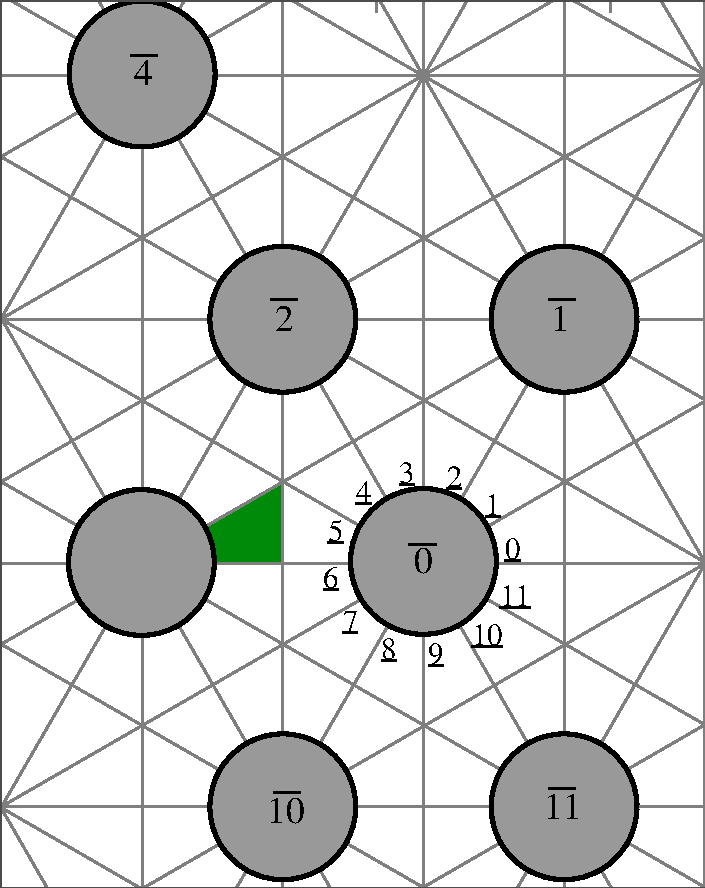
\includegraphics[width=0.45\textwidth]{diffuseFDSymbolIllustration}
\caption{\label{fig:fdflights}
Topologically distinct flights, with imposed finite horizon.
}
\end{figure}

\subsubsection{How point group changes translation}
Starting from each point on the cycle, the translation in full space is
different after completion of one cycle.


\subsubsection{Gymnastics of equations}

\Group-equivariance of the displacement in the full space.

\begin{align}
\tr{\cal L}^t &=
\sum_{\alpha \in\II_G} \tr{\cal L}_{\alpha}^t\nonumber\\
\tr{\cal L}_{\alpha}^t &=
\frac{d_\alpha}{|G|}\sum_{\sigma \in G}\sum_{h\in G}\chi_\alpha(h)
\int_{\t {\cal M}} d\tx \delta (h\tx - f^t(\tx))
e^{\beta\cdot\sigma\cdot\hphi^t(\tx)}~,
\label{e1}
\end{align}

\begin{align}
\frac{1}{\zeta_{\alpha}(\beta,s,z)} &=\exp\left(
-\frac{d_\alpha}{|G|}\sum_{\sigma\in G}\sum_{\tp}\frac{1}{n_{\tp}}
\sum_{\tx_{i}\in\tilde{p}}\sum_{r=1}^{\infty}
\frac{t_{\tp}^{r}}{r}\chi_{\alpha}(\hp^{r}(\tx_i))
e^{\beta\cdot\sigma\cdot\hat{L}_{\tp}(r,\tx_i)}
\right)
\end{align}
where we have defined
\begin{equation}
t_{\tp}\equiv \frac{z^{n_{\tp}}e^{-sT_{\tp}}}{|\ExpaEig_\tp|}
\end{equation}
and
\begin{equation}
\hat{L}_{\tp}(r,\tx_i)\equiv (e+\hp^{-1}(\tx_i)\cdots+\hp^{-r+1}(\tx_i))\cdot\hn_{\tp}(\tx_i)
\end{equation}

We are interested in the one dimensional, symmetric trivial
representation with $ d_\alpha = 1 $ and all $ \chi(h) = 1 $,; there by
we drop the subscript $ \alpha $ in the following calculation. Partial
derivative with respect to $\beta$:
\begin{align}
\frac{\partial^{2}}{\partial\beta^{2}}\frac{1}{\zeta(\beta,s,z)}
 &=\frac{1}{\zeta(\beta,s,z)}\left(\left(\frac{1}{|G|}
\sum_{\sigma\in G}\sum_{\tp}\sum_{\tx_i\in \tp}\sum_{r=1}^{\infty}\frac{\sigma\cdot \hat{L}_{\tp}(r,\tx_i)t_{\tp}^r e^{\beta\cdot\sigma\cdot \hat{L}_{\tp}(r,\tx_i)}}{n_{\tp}r}\right)^{2}\right.\nonumber\\
 & \left.-\frac{1}{|G|}\sum_{\sigma\in G}\left(\sum_{\tp}\sum_{\tx_i\in \tp}\sum_{r=1}^{\infty}\frac{\vert \sigma\cdot \hat{L}_{\tp}(r,\tx_i)\vert^{2}t_{\tp}^{r}e^{\beta\cdot\sigma\cdot \hat{L}_{\tp}(r,\tx_i)}}{n_{p}r}\right)\right).
\end{align}
The first term in the formula corresponds to $ \langle\hx\rangle^2 $ and
second to $ \langle\hx^2\rangle $


\section{Results and Discussions}

\begin{table}[htbp]
{\small
%\begin{center}
\begin{tabular}{|r|r|r|l|l|}
\hline
$\period{p}$ & \# cycles & $\zeta$(0,0) & $\lambda$ & D \\ \hline\hline
1      & 0      &   -    &   -  &   - \\
2      & 24     & -0.31697 & 1.330 & 0.375\\
3      & 64     & -0.54152 & 1.435 & 0.339\\
4      & 168    & -0.09764 & 1.902 & 0.284\\
5      & 516    &  0.02334 & 2.324 & 0.215\\
6      & 1589   & -0.00481 & 1.975 & 0.133\\
7      & 5700   & -0.01241 & 1.885 & 0.184\\
8      & 20729  & -0.01006 & 1.785 & 0.247\\ \hline\hline
\multicolumn{4}{|l|}{numerical experiment} 1.760 & 0.25 \\ \hline
\end{tabular}
\hfill
\begin{tabular}{|r|r|r|l|l|}
\hline
$\period{p}$ & \# cycles & $\zeta$(0,0) & $\lambda$ & D \\ \hline\hline
1      & 5      &   -0.2169759    &   1.39193  &   0.37795 \\
2      & 10     & -0.0248233 & 1.74541 & 0.23118\\
3      & 33     & -0.0221962 & 1.72235 & 0.25257\\
4      & 108    & -0.0002192 & 1.74450 & 0.24165\\
5      & 373    &  0.0023463 & 1.76079 & 0.24468\\
6      & 1378   &  0.0096330 & 1.75610 & 0.24068\\ \hline\hline
\multicolumn{3}{|l|}{numerical experiment}
                           & 1.760 & 0.25
\\ \hline
\end{tabular}
}

\caption{\label{TCELL2}
Results for $w$=0.3. (left) Schreiber 1992 calculation\rf{CGS92} (and
this paper) in EC. (right) Our calculation in FD. Gaspard 1992
note: ``My numerical estimate for the Lyapunov exponent when $w=0.3$ is
$\lambda = 1.760 \pm 0.002$, which supports the result of this table.''
}
\end{table}

\begin{figure}
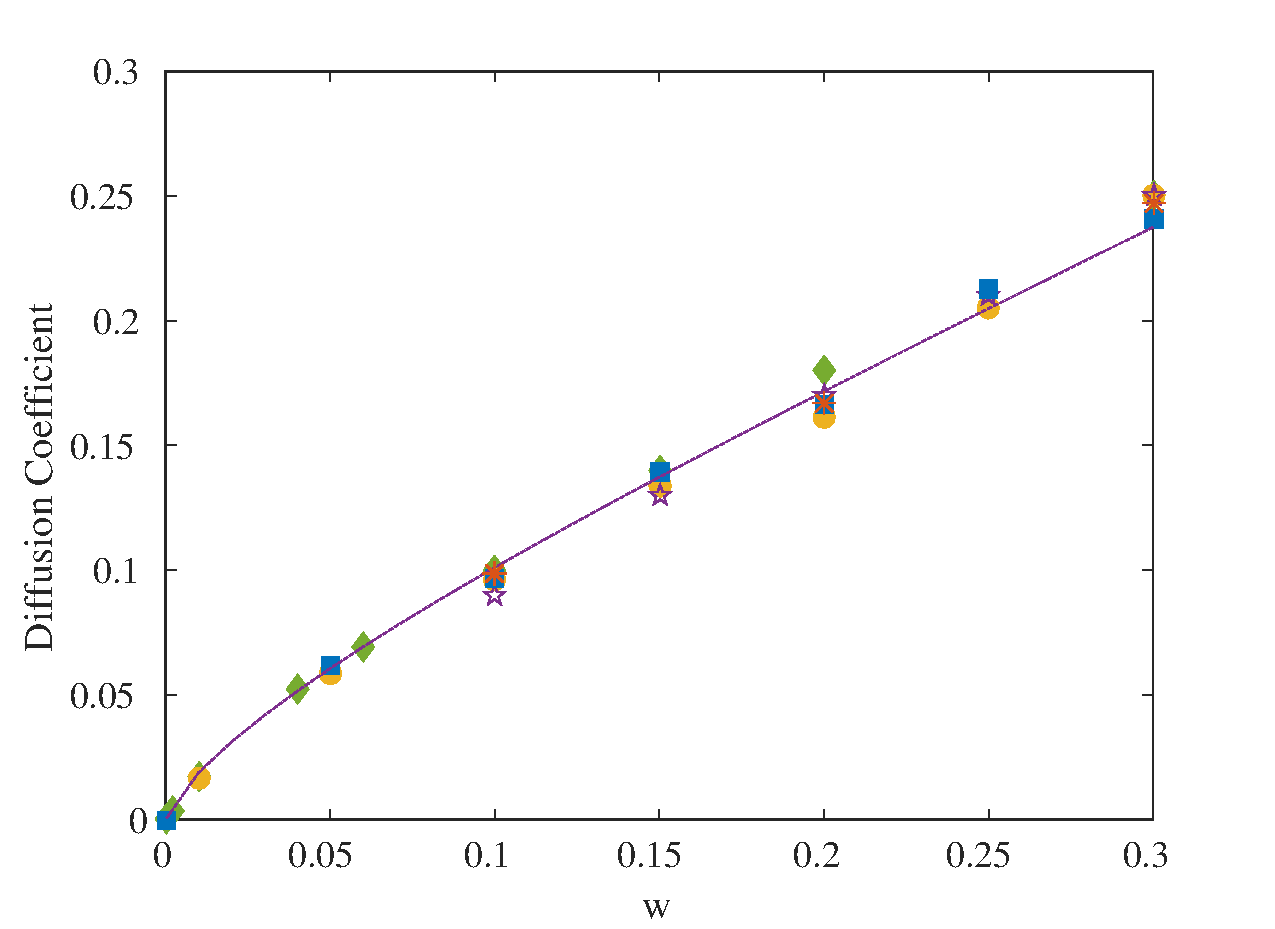
\includegraphics[width=0.5\textwidth]{diffuseDiffCoefPlot}
\caption[]{\label{fig:results}
Diffusion coefficients as a function of inter-disk separation distance
$w$.
          }
\end{figure}
% Put \label in argument of \section for cross-referencing
%\section{\label{}}

% If in two-column mode, this environment will change to single-column
% format so that long equations can be displayed. Use
% sparingly.
%\begin{widetext}
% put long equation here
%\end{widetext}

% figures should be put into the text as floats.
% Use the graphics or graphicx packages (distributed with LaTeX2e)
% and the \includegraphics macro defined in those packages.
% See the LaTeX Graphics Companion by Michel Goosens, Sebastian Rahtz,
% and Frank Mittelbach for instance.
%
% Here is an example of the general form of a figure:
% Fill in the caption in the braces of the \caption{} command. Put the label
% that you will use with \ref{} command in the braces of the \label{} command.
% Use the figure* environment if the figure should span across the
% entire page. There is no need to do explicit centering.

% \begin{figure}
% \includegraphics{}%
% \caption{\label{}}
% \end{figure}

% Surround figure environment with turnpage environment for landscape
% figure
% \begin{turnpage}
% \begin{figure}
% \includegraphics{}%
% \caption{\label{}}
% \end{figure}
% \end{turnpage}

% tables should appear as floats within the text
%
% Here is an example of the general form of a table:
% Fill in the caption in the braces of the \caption{} command. Put the label
% that you will use with \ref{} command in the braces of the \label{} command.
% Insert the column specifiers (l, r, c, d, etc.) in the empty braces of the
% \begin{tabular}{} command.
% The ruledtabular enviroment adds doubled rules to table and sets a
% reasonable default table settings.
% Use the table* environment to get a full-width table in two-column
% Add \usepackage{longtable} and the longtable (or longtable*}
% environment for nicely formatted long tables. Or use the the [H]
% placement option to break a long table (with less control than
% in longtable).
% \begin{table}%[H] add [H] placement to break table across pages
% \caption{\label{}}
% \begin{ruledtabular}
% \begin{tabular}{}
% Lines of table here ending with \\
% \end{tabular}
% \end{ruledtabular}
% \end{table}

% Surround table environment with turnpage environment for landscape
% table
% \begin{turnpage}
% \begin{table}
% \caption{\label{}}
% \begin{ruledtabular}
% \begin{tabular}{}
% \end{tabular}
% \end{ruledtabular}
% \end{table}
% \end{turnpage}

% Specify following sections are appendices. Use \appendix* if there
% only one appendix.
%\appendix
%\section{}

% If you have acknowledgments, this puts in the proper section head.
%\begin{acknowledgments}
% put your acknowledgments here.
%\end{acknowledgments}

Test of the temporary diffuse specific bibliography - \refref{RoMo08a}
is a repeat, for testing purpose only.
% Create the reference section using BibTeX:
\bibliography{../bibtex/siminos,../bibtex/diffuse}

\PublicPrivate{}{% switch \PublicPrivate{
\input ../tingnan/flotsam
      }% end \PublicPrivate{


\end{document}
%
% ****** End of file apstemplate.tex ******
